    \chapter{Especificação técnica} \label{cap:especificacao_tecnica}

\section{Análise de Contexto}

    \subsection{Visão Geral}
    O desenvolvimento deste protótipo tem a finalidade de auxiliar o professor no ensino de programação para crianças.
    
    O software, apresentado em forma de jogo com o tema reciclagem, apresentará diversos desafios em que a criança deverá solucionar criando sequências lógicas com blocos físicos. Após a ordenação dos blocos, de maneira em que achar correta, pela criança, ela deverá tirar fotos da sua solução e submetê-la para a avaliação do desafio dentro do aplicativo.
    
    Ao finalizar a captura da solução proposta, o aplicativo enviará a sequência de imagens para um servidor, hospedado na nuvem, o qual fará a análise das imagens dos blocos
    por meio de visão computacional a fim de identificar e converter os blocos em ações para o jogo.
    
    Ao final da conversão, o servidor devolverá para o jogo a solução proposta em ações.
    Caso a solução esteja correta, a criança passará para o próximo desafio, caso contrário, será oferecido uma nova tentativa.
    
    O aplicativo coletará dados durante o desafio para o preenchimento de relatórios que serão apresentados para o professor ou tutor através de um portal.
    
    A figura \ref{figura:diagrama_blocos} apresenta a visão geral do sistema proposto.
    
    \begin{figure}[h!]
        \centering
        \caption{Visão geral do sistema}
        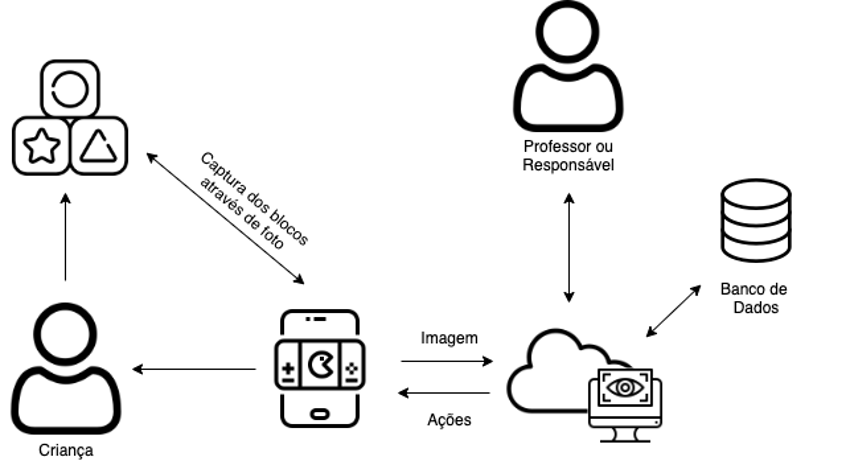
\includegraphics[width=12cm]{images/cap3/diagrama_blocos.png}
        \caption*{Fonte:o autor (2020)}
        \label{figura:diagrama_blocos}
    \end{figure}
    
    \subsection{Condições Restritivas}
    O projeto proposto apresenta algumas condições restritivas, conforme descrito
    nos próximos subitens.

        \subsubsection{Custos}
        Apesar do aplicativo jogo precisar de materiais relativamente baratos para funcionar, como blocos impressos em 3D ou até mesmo papéis coloridos dobrados de formas semelhante aos blocos impressos, ainda se faz necessário o uso de um celular com sistema operacional Android com câmera para que o aplicativo funcione. 
            
        % \subsubsection{Físicas e Ambientais}
        
        \subsubsection{Tecnológicas}
        O aplicativo jogo necessita de um celular com câmera e com o sistema operacional Android com a versão igual ou superior a 5.0- Lollipop. Por se tratar de um protótipo, o aplicativo não oferece suporte para os demais dispositivos móveis com outros sistemas operacionais, como por exemplo Iphones. 
        
        \subsubsection{Energização}
        O celular é limitado em relação à energia, tendo um período máximo que uma carga pode sustentar, esse período máximo varia conforme o modelo e o uso do dispositivo. Para diminuir os efeitos causado por essa limitação, recomenda-se o uso do aplicativo com a bateria cheia ou próximo a uma tomada caso seja necessário recarregar a bateria do dispositivo móvel.   
        
        % \subsubsection{Interferências devido ao meio}
    
    \subsection{Benefícios e Impactos}
    O aplicativo jogo apresenta alguns benefícios e impactos, conforme descrito nos próximos subitens.

        \subsubsection{Econômicos}
        Além de um celular com câmera, o aplicativo jogo proposto é capaz de funcionar com recursos relativamente baratos, como blocos impressos em 3D ou até mesmo uma folha colorida dobrada em formatos semelhantes aos cubos; o aplicativo jogo também funciona de forma simples. Portanto pode ser utilizado em casa ou implantado em escolas de forma fácil e econômica para proporcionar a crianças um contato inicial com temas como lógica de programação e sustentabilidade, além de atender às novas demandas da BNCC para o ensino.
        
        % \subsubsection{Operacionais}
        
        % \subsubsection{Estratégicos}
        
        \subsubsection{Políticos}
        A mais nova atualização da Base Nacional Comum Curricular destina uma de suas dez competência a educação integral por meio de tecnologias digitais e faz uso, no caderno de matemática, do termo “pensamento computacional”. Pensando nisso, o aplicativo jogo proposto possibilita, de uma forma simples e econômica, um meio para trabalhar essas competências nas escolas. 

        \subsubsection{Sociais}
        O aplicativo jogo apresenta benefícios sociais para as crianças, pois as crianças terão acessos a conceitos básicos de lógica de programação e oportunidade de exercitar esse conceitos, o que pode auxiliar em competências como raciocínio lógico, resolução de problemas, pensamento computacional, entre outras habilidades que tem sido cada vez mais requisitadas no mercado de trabalho. Isso sendo proporcionado por um jogo, além de gerar maior engajamento no ensino de crianças, pode desenvolver  também competências como cooperação, cumprimento de regras, controle de impulsividade, auxílio na tomada de decisões, mais facilidade para lidar com erros e fracassos entre outras habilidades sociais.
        Além disso, o aplicativo jogo, por meio do tema de reciclagem, pode desenvolver senso de sustentabilidade auxiliando na compreensão da importância do descarte correto do lixo, o que impacta direta e positivamente  o meio ambiente.

\section{Análise Funcional e de Requisitos Tecnológicos}

    \subsection{Lista de Funcionalidade e Atores}
    O sistema será composto  pelas seguintes funcionalidades:
    \begin{itemize}
        \item Desafios de lógica com o tema reciclagem;
        \item Identificação dos blocos;
        \item Conversão dos blocos em ações;
        \item Relatórios de jogo para acompanhamento do professor;
    \end{itemize}
    
    O sistema tem como atores a criança e professor/tutor.
    
    A criança é responsável pela interação com os blocos e aplicativo.
    O professor/tutor é responsável pela interação com os dados adquiridos durante a partida da criança.
    
    \subsection{Comunicação}
    A comunicação entre o aplicativo e o servidor ocorrerá de maneira unidirecional e utilizará arquitetura \textit{REST}, através da conexão Wi-Fi com a Internet.
    O aplicativo envia os dados e imagens para o servidor. Após o servidor salvar os dados e processar as imagens, ele retorna para o aplicativo.
    
        \subsubsection{REST}
        O \textit{REST (Representational State Transfer)} é uma abstração da arquitetura da \textit{Web}. Consistem em regras que permitem a criação de projetos com interfaces bem definidas, permitindo a comunicação entre aplicações.
    
    
    \subsection{Processamento}
    O processamento por parte do Software, ocorre no aplicativo e no servidor.
    O servidor recebe as imagens enviadas pelo aplicativo e passa cada uma pelo algoritmo de visão computacional, responsável pela identificação de cada bloco nas fotos. Após a identificação dos blocos, ele salva no banco de dados e retorna para o aplicativo as ações a serem executadas.
    O aplicativo captura as imagens e as envia para o servidor através da Internet. Após o processamento no servidor, o aplicativo recebe as ações e as transforma em trechos de código para ser executados durante o jogo.
    % Precisa escrever sobre o processamento das imagens, qual tipo de modelo, biblioteca, linguagem etc.
    
    \subsection{Interface Homem-Máquina}
    As interações da criança será com os blocos físicos e com o aplicativo.
    Na tela inicial, é apresentado duas opções, créditos e desafios, como mostra a figura \ref{figura:tela_inicial}.
    
    \begin{figure}[h!]
        \centering
        \caption{Tela Inicial}
        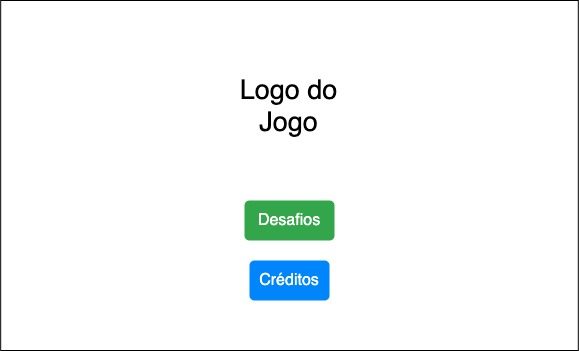
\includegraphics[width=12cm]{images/cap3/Tela Inicial.jpg}
        \caption*{Fonte:o autor (2020)}
        \label{figura:tela_inicial}
    \end{figure}
    
    Ao acessar a opção de desafios é apresentado a lista de todos os desafios disponíveis, juntamente com o progresso de cada desafio (se disponível), conforme apresentado na figura \ref{figura:tela_desafios}
    
    \begin{figure}[h!]
        \centering
        \caption{Tela de Desafios}
        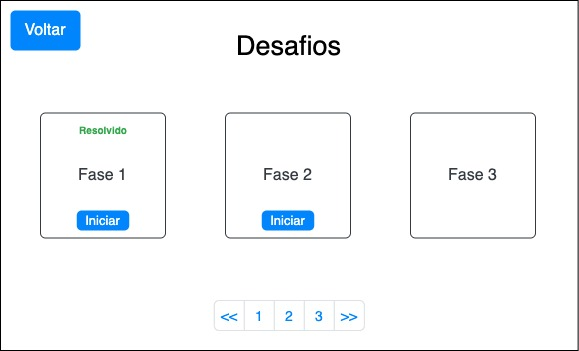
\includegraphics[width=12cm]{images/cap3/tela_desafios.jpg}
        \caption*{Fonte:o autor (2020)}
        \label{figura:tela_desafios}
    \end{figure}
    
    Nessa tela, é possível ver a lista de desafios, um desafio só poderá ser iniciado caso o anterior tenha sido resolvido.
    É possível clicar no botão voltar para retornar a tela anterior.
    Ao clicar no botão iniciar do desafio, a criança poderá ser direcionada para a tela de cadastro ou direto para a tela do desafio.
    Caso a criança não tenha preenchido as informações para identificá-la, essas informações serão coletadas em uma tela específica, conforme figura \ref{figura:cadastro}. Caso contrario ela é direcionada para a tela que contém o desafio a ser solucionado.
    
    \begin{figure}[h!]
        \centering
        \caption{Tela de Cadastro}
        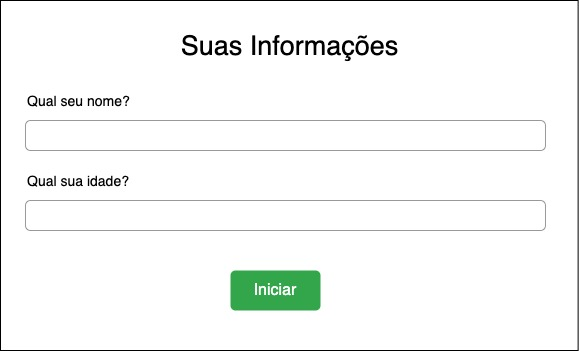
\includegraphics[width=12cm]{images/cap3/informacoes_usuario.jpg}
        \caption*{Fonte:o autor (2020)}
        \label{figura:cadastro}
    \end{figure}
    
    A figura \ref{figura:tela_jogo} mostra a interface principal durante o jogo.
    
    \begin{figure}[h!]
        \centering
        \caption{Tela do Jogo}
        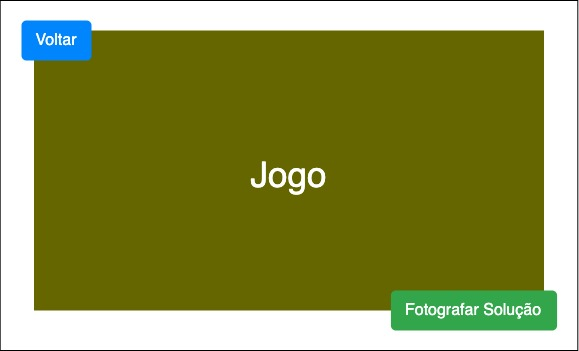
\includegraphics[width=12cm]{images/cap3/tela_jogo.jpg}
        \caption*{Fonte:o autor (2020)}
        \label{figura:tela_jogo}
    \end{figure}
    
    Nessa tela é possível executar duas ações.
    Clicando no botão voltar, a criança é redirecionada para a lista de desafios.
    Selecionando o botão Fotografar Solução, é aberto uma janela, conforme figura \ref{figura:fotografar_blocos} para fotografar a solução.
    
    \begin{figure}[h!]
        \centering
        \caption{Tela para fotografar solução}
        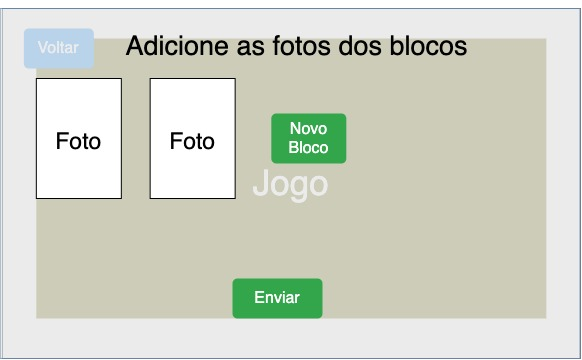
\includegraphics[width=12cm]{images/cap3/Fotografar_blocos.jpg}
        \caption*{Fonte:o autor (2020)}
        \label{figura:fotografar_blocos}
    \end{figure}
    
    Cada bloco deve ser fotografado e adicionado utilizando o botão Novo Bloco.
    Ao fotografar todos os blocos, pode-se clicar no botão enviar para que a solução seja processada.
    Após a conversão das fotos em ações para o jogo, o usuário é direcionado para a tela de jogo, onde as ações convertidas serão executadas.
    Caso a solução seja a correta e o personagem chegue na lixeira correta, será apresentado uma mensagem de sucesso, conforme figura \ref{figura:solucao_correta}. Caso contrário, será apresentado a mensagem de falha, permitindo uma nova tentativa, figura \ref{figura:solucao_incorreta}.
    
    \begin{figure}[h!]
        \centering
        \caption{Mensagem de solução correta}
        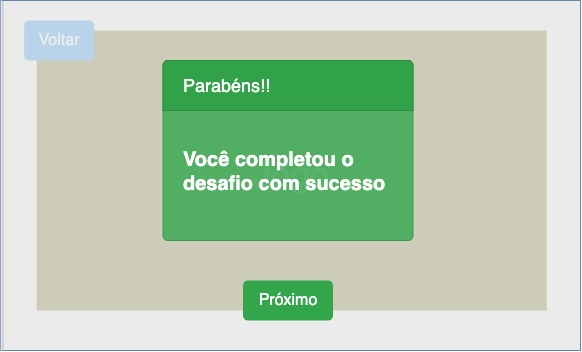
\includegraphics[width=12cm]{images/cap3/solucao_correta.jpg}
        \caption*{Fonte:o autor (2020)}
        \label{figura:solucao_correta}
    \end{figure}
    
    \begin{figure}[h!]
        \centering
        \caption{Mensagem de solução incorreta}
        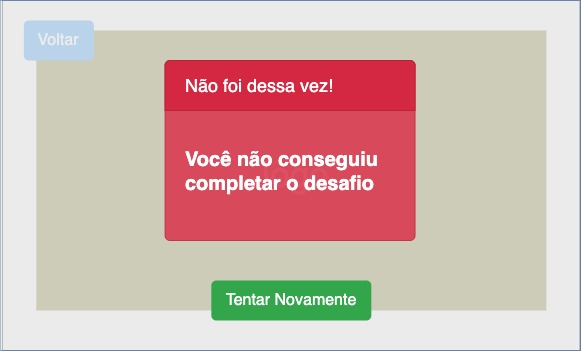
\includegraphics[width=12cm]{images/cap3/solucao_incorreta.jpg}
        \caption*{Fonte:o autor (2020)}
        \label{figura:solucao_incorreta}
    \end{figure}
    
    
    \subsection{Sistemas Controlados Automaticamente}
    O Sistema não apresentará sistemas controlados automaticamente.
    
    \subsection{Aquisição de dados e Atuação}
    A coleta das fotos se dará através da ação da criança que está jogando. Após concluir a proposta de solução do desafio, a mesma deve capturar sua proposta utilizando a câmera do dispositivo móvel.
    Após a captura das imagens a criança, utilizando um botão de envio, enviará as fotos para o servidor, onde as fotos serão processadas e transformadas em ações para o jogo.
    
    O envio das fotos e o recebimento da conversão em ações do jogo é realizado através de conexão com a Internet.
    Toda proposta de solução, esteja ela correta ou não, será salva no banco de dados, após sua interpretação, para gerar relatórios estatísticos.


\section{Análise da Arquitetura do Sistema}

    \subsection{Hardware}
    O hardware do sistema será composto por blocos físicos e o dispositivo mobile com câmera.
    
    Os blocos físicos serão construídos de PLA, impressos em 3D, com o tamanho aproximado de 10cm x 10cm x 5cm, seus cantos serão arredondados para evitar acidentes no manuseio. Para facilitar a identificação, além da sua cor, cada bloco possuirá um simbolo representado o tipo da ação.
    
    O dispositivo mobile deverá ser um celular \textit{Android} com câmera, podendo variar entre os modelos existentes no mercado.
    
    \subsection{Software}
     No tópico a seguir, são apresentados os diagramas do software.
        
        \subsubsection{DER/MER}
        O diagrama apresentado na figura \ref{figura:der_mer} mostra os relacionamentos entre os objetos do sistema, juntamente com seus atributos.
        
        \begin{figure}[h!]
            \centering
            \caption{Use Case}
            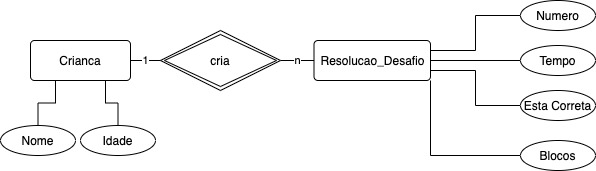
\includegraphics[width=12cm]{images/cap3/MER_DER.jpg}
            \caption*{Fonte:o autor (2020)}
            \label{figura:der_mer}
        \end{figure}
        
        O banco de dados possuirá dois esquemas de documentos, um para representar a criança e outro para representar a resolução do desafio.
        O esquema da criança, possui obrigatoriamente os atributos de Nome e Idade, podendo ser complementado com mais informações caso necessário.
        O esquema para a resolução do desafio, possui os seguintes atributos:
        
        \begin{itemize}
            \item Numero, representando o numero do desafio.
            \item Tempo, representando o tempo que a criança levou para submeter a solução.
            \item Esta Correta, representando se a solução apresentada está correta ou não.
            \item Blocos, representando os blocos que foram utilizados.
        \end{itemize} 
        
        \subsubsection{Use Case}
        O Aplicativo conta com funções de identificação da criança (Perfil), Inicio de desafio e submissão de solução, conforme apresentado no diagrama de caso de uso na figura \ref{figura:use_case}.
        
        \begin{figure}[h!]
            \centering
            \caption{Use Case}
            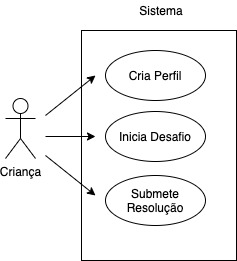
\includegraphics[width=8cm]{images/cap3/Use Case.jpg}
            \caption*{Fonte:o autor (2020)}
            \label{figura:use_case}
        \end{figure}
        
        \subsubsection{Diagramas de Sequência}
        
        Nesse tópico será apresentado os diagramas de sequencia para as funcionalidades principais do aplicativo.
        
        \subsubsubsection{Criação de Perfil}
        
        A figura \ref{figura:sequencia_perfil} mostra o diagrama de sequência para a realização do cadastro de informações da criança. Todas as informações são salvas localmente e em um banco de dados na nuvem.
        
        \begin{figure}[h!]
            \centering
            \caption{Diagrama de Sequência - Perfil}
            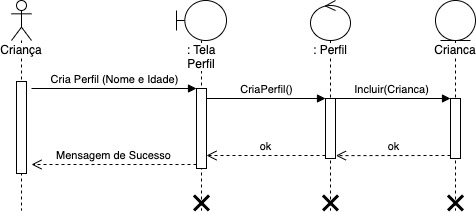
\includegraphics[width=12cm]{images/cap3/Sequencia_Perfil.jpg}
            \caption*{Fonte:o autor (2020)}
            \label{figura:sequencia_perfil}
        \end{figure}
        
        \subsubsubsection{Submissão da Resolução}
        
        O diagrama apresentado na figura \ref{figura:sequencia_jogo} mostra o processo de submissão da solução e validação da mesma.
        
        \begin{figure}[h!]
            \centering
            \caption{Diagrama de Sequência - Submissão da Resolução}
            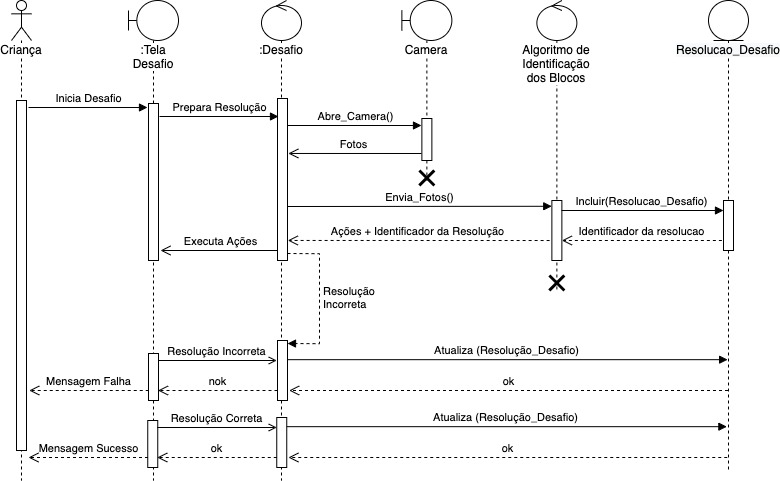
\includegraphics[width=14cm]{images/cap3/Sequencia_Jogo.jpg}
            \caption*{Fonte:o autor (2020)}
            \label{figura:sequencia_jogo}
        \end{figure}
        
        Ao iniciar o desafio, a data e hora são salvos localmente para que, quando a resolução for submetida, essa informação seja salva junto com as demais no banco de dados.
        Após o aplicativo processar as ações convertidas pelo algoritmo de identificação dos blocos, o aplicativo valida a solução e atualiza a resolução no banco com o seu status, correto ou não correto.
        
        
   